\frontmatter

%\begin{center}
% Here begins the title page
\vspace{10mm}
\title{\normalsize

%
% The DTU Physics logo to the left and the DTU logo to the right
\noindent
\begin{minipage}[b]{20mm} 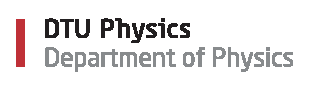
\includegraphics[height=10mm]{figs/chap00/DTU_Physics_logo.eps}\\[-1.5mm] \end{minipage}
\hfill 
\includegraphics[height=15mm]{figs/chap00/DTULogo.eps} \\[10mm]
%
% Identification of the thesis
{\normalsize Bachelor/Master/Ph.D. Thesis}\\[12mm]
%
% The title of the thesis
{\bf\Huge This is a fine title}\\[10mm]
%
% Author(s), picture, affiliation
{\Large Firstname Lastname}\\
s06xxxx\\[15mm]
%
\rule{\textwidth}{0.5pt}\\[5mm]          % A ruler
\centerline{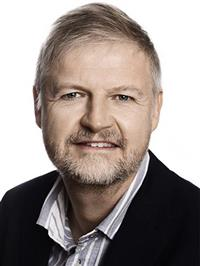
\includegraphics[height=60mm]{figs/chap00/FrontFig.eps}} % A picture
\rule{\textwidth}{0.5pt}\\[15mm]         % A ruler
Supervisor: Henrik Bruus\\[5mm]          % The supervisor
Department of Physics\\                  % The department
Technical University of Denmark\\[3mm]   % The university
%
8 February 2016                         % The date
\date{}
} % Here ends the title page

\maketitle
% Generate the title page

%\end{center}


% Now comes abstract, resume, and preface

\chapter*{Abstract}
\markboth{ABSTRACT}{ABSTRACT}
This is the abstract of the entire thesis
\\[20mm]

\chapter*{Resum\'e}
\markboth{RESUME}{RESUME}
Dette er et dansk resum\'e af afhandlingen
\\[20mm]

\chapter*{Preface}
\markboth{PREFACE}{PREFACE}
This is the preface to the thesis
\\[15mm]

\begin{center}
\emph{signature}\\[2mm]
Firstname Lastname\\
Department of Physics\\
Technical University of Denmark\\
8 February 2016 
\end{center}

% Here comes the table of contents

\tableofcontents

% Here comes list of figures, tables, and symbols


\listoffigures
\addcontentsline{toc}{chapter}{List of figures}

\listoftables
\addcontentsline{toc}{chapter}{List of tables}

\chapter*{List of symbols}
\markboth{LIST OF SYMBOLS}{LIST OF SYMBOLS}
\addcontentsline{toc}{chapter}{List of symbols}
\begin{center}
\begin{tabular}{p{2cm}p{6cm}p{3cm}}
Symbol                          & Description                      & Unit \\
\hline\hline
$\rho$                          & Mass density                     & kg m$^{-3}$ \\
$\boldsymbol{x}$                & Position vector                  & m \\
$\boldsymbol{v}$                & Velocity vector                  & m s$^{-1}$ \\
$v$                             & Velocity                         & m s$^{-1}$ \\
$\boldsymbol{\sigma}$           & Cauchy stress tensor             & N m$^{-2}$ \\
$\boldsymbol{f}$                & Body force density               & N m$^{-3}$ \\
$\boldsymbol{g}$                & Gravity                          & N kg$^{-1}$ \\
$\boldsymbol{n}$                & Surface outward normal vector    & \\
$p$                             & Pressure                         & N m$^{-2}$ \\
$\boldsymbol{\tau}$             & Deviatoric stress tensor         & N m$^{-2}$ \\
$\dot{\boldsymbol{\gamma}}$     & Strain rate                      & s$^{-1}$ \\
$\dot{\boldsymbol{\gamma}}^{\mathrm{dev}}$ & Deviatoric strain rate & s$^{-1}$ \\
$\mu$                           & Dynamic viscosity                & kg m$^{-1}$ s$^{-1}$ \\
$\dot{\boldsymbol{\gamma}}$     & Strain rate                      & s$^{-1}$ \\
$\mathcal{U}$                   & Total energy per unit mass       & J kg$^{-1}$ \\
$\boldsymbol{q}$                & Heat flux                        & J m$^{-2}$ \\
$T$                             & Temperature                      & K \\
$k$                             & Thermal conductivity             & J K$^{-1}$ m$^{-1}$ \\
$q$                             & Heat source density              & J m$^{-3}$ s$^{-1}$ \\
$G$                             & Pressure gradient [in Poiseuille flow] & N m$^{-3}$ \\
$Q$                             & Volume flow rate                 & m$^3$ s$^{-1}$ \\
\hline
$\mathcal{L}$                   & Differential operator            & \\
$u$                             & Solution to scalar problem       & \\
$f$                             & Source term                      & \\
$\Omega$                        & Computational domain             & \\
$\partial\Omega$                & Domain boundary                  & \\
$h$                             & Mesh size                        & \\
$\mathbb{H}$                    & Function space                   & \\
$\mathbb{H}_m$                  & $m$ dimensional function space   & \\
$v,w,\varphi$                   & Members of function space        & \\
$\langle\cdot\,\cdot\rangle$    & Inner product                    & \\
$p$                             & Accuracy                         & \\
$q$                             & Smoothness                       & \\
\end{tabular}
\end{center}


\mainmatter % And finally, we move on to the first chapter
